\section[Gleichstellungsbüro am FB11]{Gleichstellung betrifft uns ALLE – Das Gleichstellungsbüro stellt sich vor}
\begin{minipage}{0.1\textwidth}
    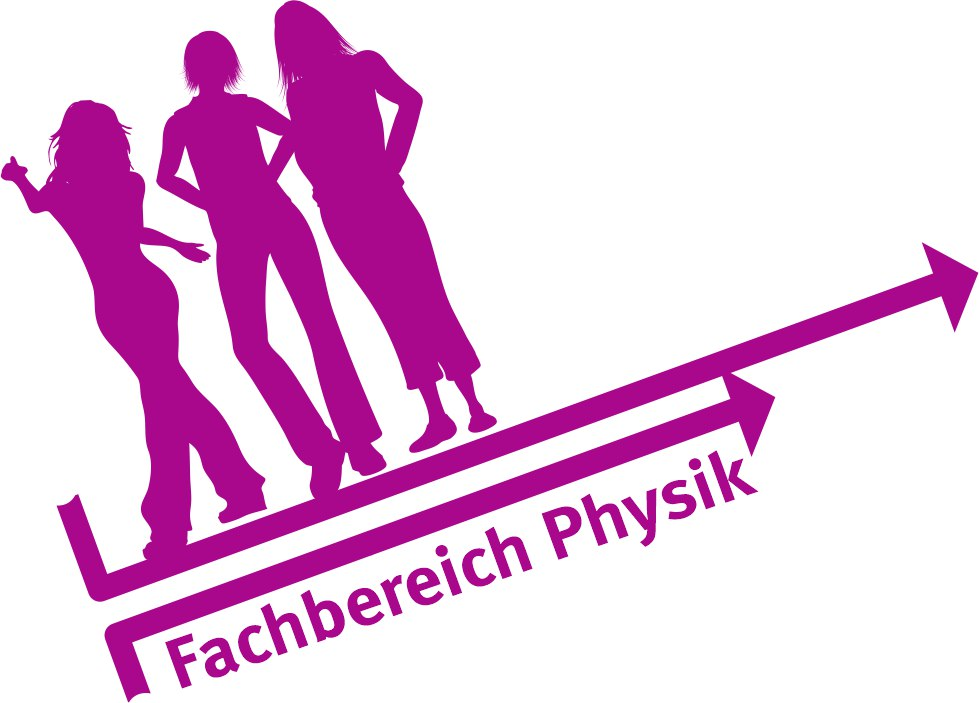
\includegraphics[width=\textwidth]{res/gst_buero.jpg}
\end{minipage}\hfill
\begin{minipage}{0.75\textwidth}
    \centering
    \textbf{Auch das Gleichstellungsbüro des Fachbereichs möchte Euch herzlich an der WWU und am Fachbereich begrüßen.}
\end{minipage}\hfill
\begin{minipage}{0.1\textwidth}
    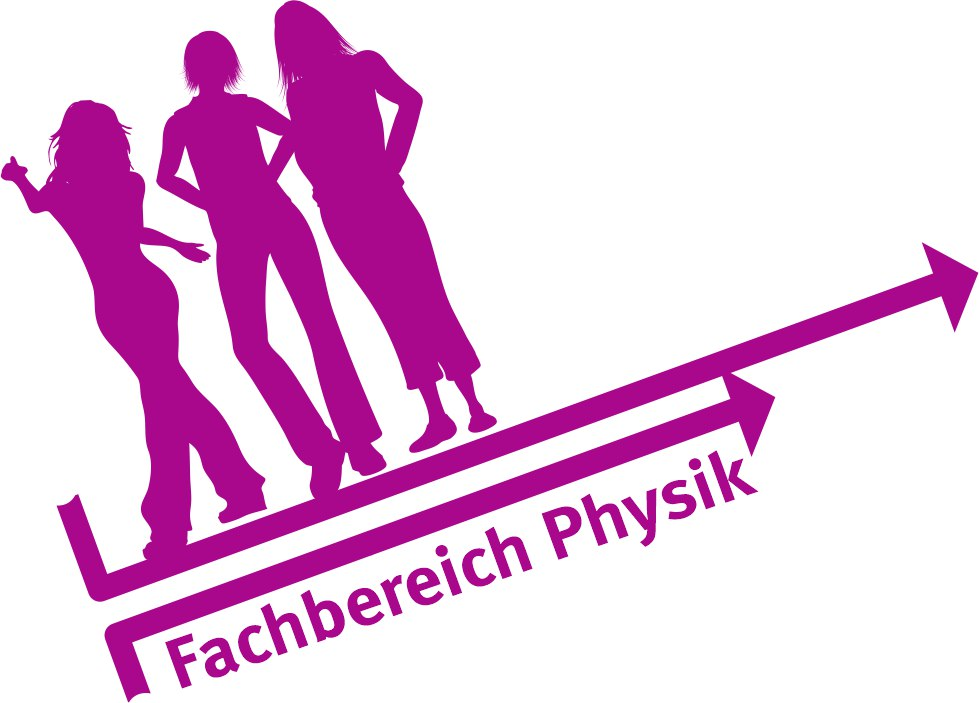
\includegraphics[width=\textwidth]{res/gst_buero.jpg}
\end{minipage}

\begin{multicols}{2}
Die ersten Veranstaltungen der O-Woche sind schon vorbei, alles ist neu. Der Hörsaal schaut ganz anders aus als ein Klassenzimmer und sicherlich habt ihr auch schon eure ganzen Mitstudierenden gesehen, die, genau wie ihr, gerade einen neuen Lebensabschnitt mit dem Studium der Physik beginnen. Doch habt ihr mal darauf geachtet, wie die Verteilung der Geschlechter ausschaut? Wenn nicht, probiert es mal! Ihr werdet feststellen, dass vor allem Männer stark vertreten sind. Die Anzahl der weiblichen Physikerinnen nimmt entsprechend des Kaskadenprinzips mit steigenden Karrierestufen sogar immer weiter ab: Es gibt noch weniger Doktorandinnen, weibliche Post-Docs und noch weniger Profesorinnen. Warum ist das so? Welches strukturelle Problem liegt dem zugrunde? Und was können wir dafür tun, um den Frauenanteil in der Physik zu erhöhen? An wen wende ich mich bei sexueller Belästigung im Studium? Für alle diese Fragen sind wir vom Gleichstellungsbüro zuständig. \\

Zum Beispiel veranstalten wir regelmäßig Gender Breakfast Talks und Physikerinnen-Cafés. Dort können wir uns austauschen und unterstützen sowie über interessante und aktuelle Themen quatschen. Der Gender Breakfast Talk ist eine Veranstaltung explizit für alle Geschlechter – Gleichstellung ist nämlich kein Thema für Frauen allein. Während des Physikerinnen Cafés möchten wir jedoch eine für Frauen geschützte Umgebung schaffen und Hürden und Probleme besprechen, die speziell Frauen im Studium und in der Karriere begegnen. \\

Beim Gender Breakfast Talk starten wir immer mit einem wissenschaftlichen Input-Talk Gleichstellungmit neusten Ergebnissen aus der Gender & MINT Forschung. Dazu laden wir eine Rednerin ein, die in diesem Gebiet forscht. So bekommt jede:r Zuhörende die Möglichkeit, die eigenen Gender-Kompetenzen auszubauen – keine Angst, Vorkenntnisse werden nicht benötigt. Wichtig ist uns dabei, dass der Talk wissenschaftlich ist. Das bedeutet, dass alle Aussagen auf Studien beruhen und fundiert sind. Dementsprechend wollen wir eine offene und vielseitige Diskussion führen, was auch bedeutet, dass wir uns kritisch hinterfragen. Danach sprechen wir über das Thema des Vortrags oder auch jedes andere Thema, das aufkommt, klären Fragen und teilen unsere Erfahrungen in bestimmten Situationen. Dazu gibt es auch noch ein kleines kostenloses Frühstück. \\

Das Physikerinnen-Café findet immer statt, wenn im Allgemeinen Physikalischen Kolloquium eine Rednerin spricht. Am selben Tag ihres Vortrags treffen wir uns vorab und sprechen sowohl über ihren Karriereweg als auch über geschlechterbezogene Probleme, denen sie während ihres eigenen Werdegangs begegnet ist. Meistens haben diese schon weiter fortgeschrittenen Wissenschaftlerinnen super Tipps für uns Studentinnen. \\

Auch für die Themen sexualisierte Diskriminierung, Belästigung und Gewalt sind wir zuständig. Dabei haben wir immer ein offenes Ohr für euch, gehen mit euren Sorgen sowie Nöten diskret um und kennen die nötigen Ansprechpersonen, wenn weitere Schritte eingeleitet werden sollen. \\

Alle Infos dafür findet ihr auf unserer Website \footnote{\url{www.uni-muenster.de/Physik/department/equality/}} oder bekommt ihr regelmäßig, indem ihr euch auf unseren entspannten Newsletter setzt. Dies geht ganz einfach über diesen QR-Code: \\
\begin{center}
    
\includegraphics[width=\columnwidth]{res/gst_QR.png} %Newsletter QR-Code
\end{center}

Grundsätzlich gilt: Wir sind die ersten Ansprechpersonen, wenn es um Gleichstellungsthemen geht. Also ruft uns einfach an (251 83-33516), schreibt uns eine E-Mail (\textbf{\email{gleichstellung.physik@uni-muenster.de}}) oder kommt auf einen Kaffee rum (Raum: AP106) und wir helfen euch. \\


\fibelsig{Anna Niemann und Janice Bode}
\end{multicols}


